\documentclass[notheorems]{beamer}
% bibliography
\usepackage[backend=biber]{biblatex}
\bibliography{ref.bib}


\usepackage{../../template/sty/packages_math}
\usepackage{../../template/sty/packages_formatting}
\usepackage{../../template/sty/shortcuts_pm}
\usepackage{../../template/sty/beamer-template}

\graphicspath{{../expe/}}


%%%%%% Pink beamer colour theme
%% https://www.r-bloggers.com/create-your-own-beamer-template/

%%%% COLOURS

%\definecolor{CaPink}{RGB}{232, 94, 138} % default pink
%\definecolor{CaDarkUnsatPink}{RGB}{249, 26, 97} % dark unsaturated pink
%\definecolor{CaLightPink}{RGB}{253, 175, 200} % light pink
%\definecolor{CaRed}{RGB}{223, 47, 81} % red

\definecolor{CaDarker}{HTML}{C86FC9}
\definecolor{CaDark}{HTML}{E085CE}
\definecolor{CaNormal}{HTML}{F79AD3}
\definecolor{CaLight}{HTML}{F7C7DB}


%%%% THEME


\setbeamercolor{palette primary}{bg=CaDarker,fg=white}
\setbeamercolor{palette secondary}{bg=CaDark,fg=white}
\setbeamercolor{palette tertiary}{bg=CaNormal,fg=white}
\setbeamercolor{palette quaternary}{bg=CaLight,fg=white}

%% header color
% https://tex.stackexchange.com/questions/321097/how-to-change-color-of-shadow-around-frametitle-latex-beamer
\pgfdeclarehorizontalshading[frametitle.bg,frametitle right.bg]{beamer@frametitleshade}{\paperheight}{
    color(0pt)=(CaDarker);
    color(\paperwidth)=(CaDarker)}

\setbeamercolor{normal text}{fg = black}

\setbeamercolor{frametitle}{fg = white, bg = CaDarker}
\setbeamercolor{title}{fg = white, bg = CaDarker}
\setbeamercolor{subtitle}{fg = white, bg = CaDark}

\setbeamercolor{author in head/foot}{fg = white, bg = CaDarker}
\setbeamercolor{title in head/foot}{fg = white, bg = CaDarker}
\setbeamercolor{numbering in head/foot}{fg = white, bg = CaDarker}
\setbeamercolor{date in head/foot}{fg = white, bg = CaDarker}

\setbeamercolor{section in toc}{fg = CaDark}
\setbeamercolor{section in toc shaded}{fg = CaDark}

\setbeamercolor{item}{fg = CaDarker}
\setbeamercolor{subitem}{fg = CaNormal}
\setbeamercolor{subsubitem}{fg = CaLight}
\setbeamercolor{description item}{fg = CaNormal}

\setbeamercolor{bibliography entry author}{fg = CaNormal}
\setbeamercolor{bibliography entry title}{fg = black}
\setbeamercolor{bibliography entry note}{fg = CaDarker}

\setbeamercolor{footnote mark}{fg = CaDarker}

%\setbeamercolor{caption}{fg = white}
\setbeamercolor{caption name}{fg = CaDarker}
\setbeamercolor{caption source}{fg = CaDark}

% % Standard block
% \setbeamercolor{block title}{fg = white, bg = green!20!blue}
% \setbeamercolor{block body}{bg = blue!1!white}
%
% % Alert block
% \setbeamercolor{block title alerted}{fg = white, bg = red}
% \setbeamercolor{block body alerted}{bg = red!1!white}
%
% % Example block
% \setbeamercolor{block title example}{fg = white, bg = green!80!blue}
% \setbeamercolor{block body example}{bg = green!1!white}



%%%%%%% Pink beamer colour theme
%% https://www.r-bloggers.com/create-your-own-beamer-template/

%%%% COLOURS

%\definecolor{CaPink}{RGB}{232, 94, 138} % default pink
%\definecolor{CaDarkUnsatPink}{RGB}{249, 26, 97} % dark unsaturated pink
%\definecolor{CaLightPink}{RGB}{253, 175, 200} % light pink
%\definecolor{CaRed}{RGB}{223, 47, 81} % red

\definecolor{CaDarker}{HTML}{C86FC9}
\definecolor{CaDark}{HTML}{E085CE}
\definecolor{CaNormal}{HTML}{F79AD3}
\definecolor{CaLight}{HTML}{F7C7DB}


%%%% THEME


\setbeamercolor{palette primary}{bg=CaDarker,fg=white}
\setbeamercolor{palette secondary}{bg=CaDark,fg=white}
\setbeamercolor{palette tertiary}{bg=CaNormal,fg=white}
\setbeamercolor{palette quaternary}{bg=CaLight,fg=white}

%% header color
% https://tex.stackexchange.com/questions/321097/how-to-change-color-of-shadow-around-frametitle-latex-beamer
\pgfdeclarehorizontalshading[frametitle.bg,frametitle right.bg]{beamer@frametitleshade}{\paperheight}{
    color(0pt)=(CaDarker);
    color(\paperwidth)=(CaDarker)}

\setbeamercolor{normal text}{fg = black}

\setbeamercolor{frametitle}{fg = white, bg = CaDarker}
\setbeamercolor{title}{fg = white, bg = CaDarker}
\setbeamercolor{subtitle}{fg = white, bg = CaDark}

\setbeamercolor{author in head/foot}{fg = white, bg = CaDarker}
\setbeamercolor{title in head/foot}{fg = white, bg = CaDarker}
\setbeamercolor{numbering in head/foot}{fg = white, bg = CaDarker}
\setbeamercolor{date in head/foot}{fg = white, bg = CaDarker}

\setbeamercolor{section in toc}{fg = CaDark}
\setbeamercolor{section in toc shaded}{fg = CaDark}

\setbeamercolor{item}{fg = CaDarker}
\setbeamercolor{subitem}{fg = CaNormal}
\setbeamercolor{subsubitem}{fg = CaLight}
\setbeamercolor{description item}{fg = CaNormal}

\setbeamercolor{bibliography entry author}{fg = CaNormal}
\setbeamercolor{bibliography entry title}{fg = black}
\setbeamercolor{bibliography entry note}{fg = CaDarker}

\setbeamercolor{footnote mark}{fg = CaDarker}

%\setbeamercolor{caption}{fg = white}
\setbeamercolor{caption name}{fg = CaDarker}
\setbeamercolor{caption source}{fg = CaDark}

% % Standard block
% \setbeamercolor{block title}{fg = white, bg = green!20!blue}
% \setbeamercolor{block body}{bg = blue!1!white}
%
% % Alert block
% \setbeamercolor{block title alerted}{fg = white, bg = red}
% \setbeamercolor{block body alerted}{bg = red!1!white}
%
% % Example block
% \setbeamercolor{block title example}{fg = white, bg = green!80!blue}
% \setbeamercolor{block body example}{bg = green!1!white}

%%%%% INFORMATION

\title{Machine Learning Décentralisé Respectueux de la Vie Privée}
\author{Paul Mangold}


\date{Journée RIC \\[1em]
  1er Octobre 2020}

%%%%% DOCUMENT

\begin{document}

%% TITLE PAGE

\begin{notitle}
  \begin{frame}
    \titlepage
  \end{frame}
  \addtocounter{framenumber}{-1}
\end{notitle}

\section{Introduction}
\subsection{Magnet}
\begin{frame}
  Je suis doctorant dans l'équipe Magnet \footcite{magnet} d'Inria, avec Aurélien Bellet \footcite{abellet} et Marc Tommasi \footcite{mtommasi}.

  \vspace{1em}

  Magnet se concentre sur :
  \begin{itemize}
  \item machine learning décentralisé ;
  \item respect de la vie privée ;
  \item traitement de la parole ;
  \item graphes et traitement de la langue : apprentissage semi supervisé, apprentissage de représentation ;
  \item équité en apprentissage.
  \end{itemize}
\end{frame}

\section{Machine Learning Centralisé}

\subsection{Apprentissage Supervisé}
\begin{frame}
  Apprentissage supervisé :
  \begin{itemize}
  \item $X$ : ensemble de variables (features) ;
  \item $Y$ : labels.
  \end{itemize}

  Objectif : prédire les labels en fonction des features.

  \vspace{0.5em}

  $\longrightarrow$ On cherche un modèle $h_w$ tel que $h_w(x) \approx y$ pour tous les éléments du dataset.
\end{frame}

\begin{frame}
  Pour évaluer le modèle on définit la fonction :
  \begin{align}
    \mathcal L(w; X, Y) = \frac 1 n \sum_{i=1}^n (h_w(x_i) - y_i)^2,
  \end{align}

  minimale quand le modèle est bon.

  \vspace{1em}

  $\longrightarrow$ Il ne reste plus qu'à trouver ce minimum !
\end{frame}

\subsection{Descente de Gradient}
\begin{frame}
  \centering
  \vspace{1.7em}
  Choisir un point de départ $w_0$.

  \vspace{-3.37em}

  
\includegraphics[width=0.8\linewidth]{images/gd_1.pdf}
\end{frame}
\addtocounter{framenumber}{-1}
\begin{frame}
  \begin{align}
    w_{t+1} = w_t - \gamma \nabla \mathcal L(w; X, Y) \nonumber
  \end{align}

  \vspace{-4em}

  \centering

  
\includegraphics[width=0.8\linewidth]{images/gd_2.pdf}
\end{frame}
\addtocounter{framenumber}{-1}
\begin{frame}
  \begin{align}
    w_{t+1} = w_t - \gamma \nabla \mathcal L(w; X, Y) \nonumber
  \end{align}

  \vspace{-4em}

  \centering

  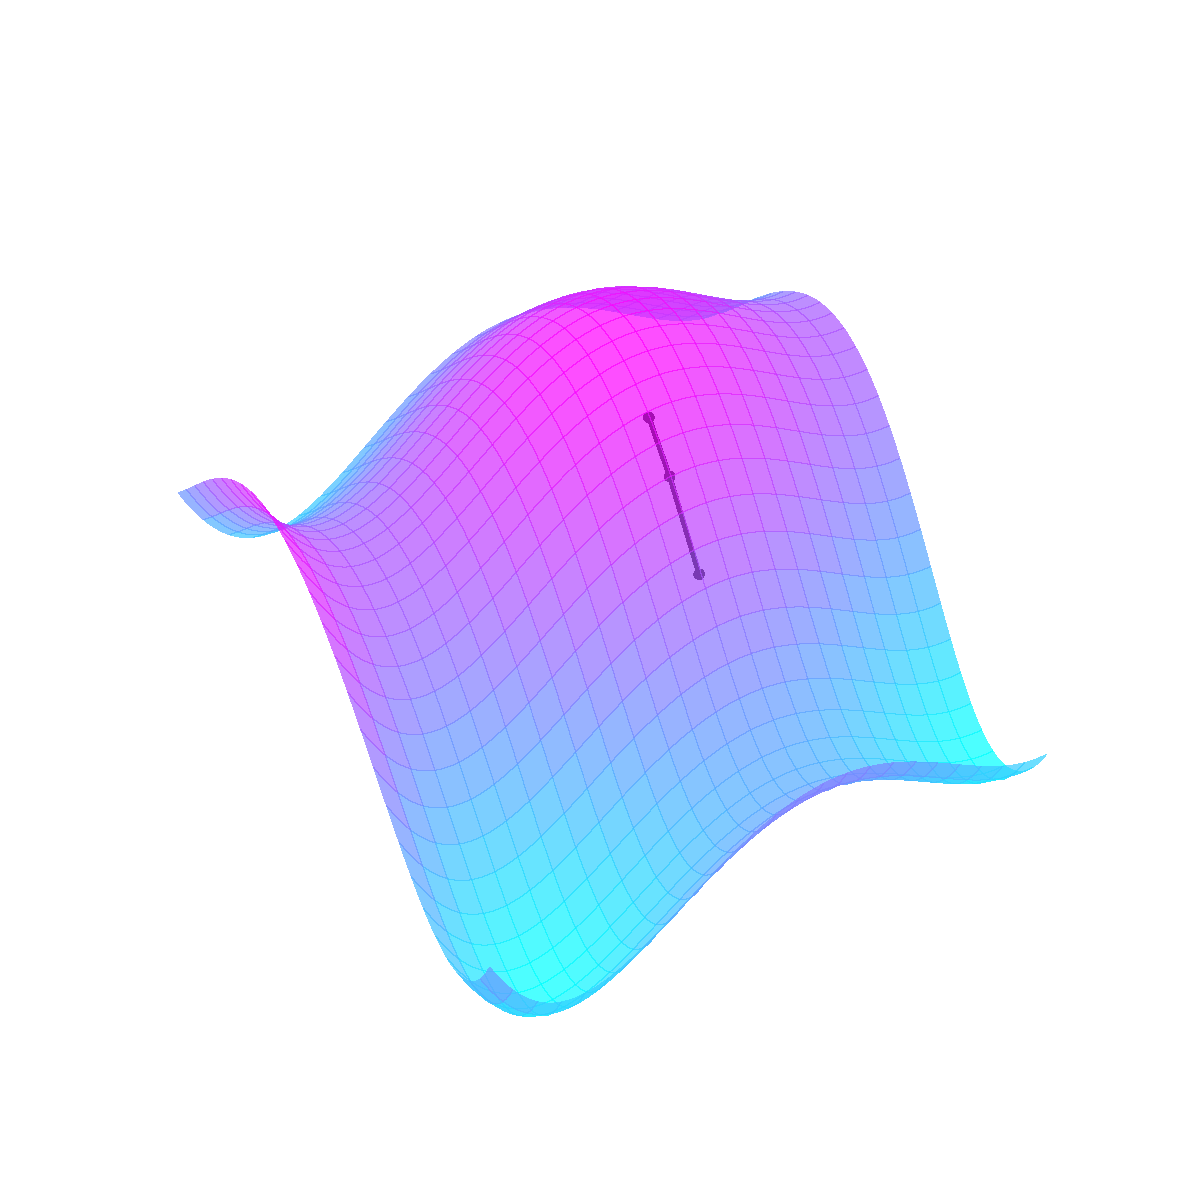
\includegraphics[width=0.8\linewidth]{images/gd_3.pdf}
\end{frame}
\addtocounter{framenumber}{-1}
\begin{frame}
  \begin{align}
    w_{t+1} = w_t - \gamma \nabla \mathcal L(w; X, Y) \nonumber
  \end{align}

  \vspace{-4em}

  \centering

  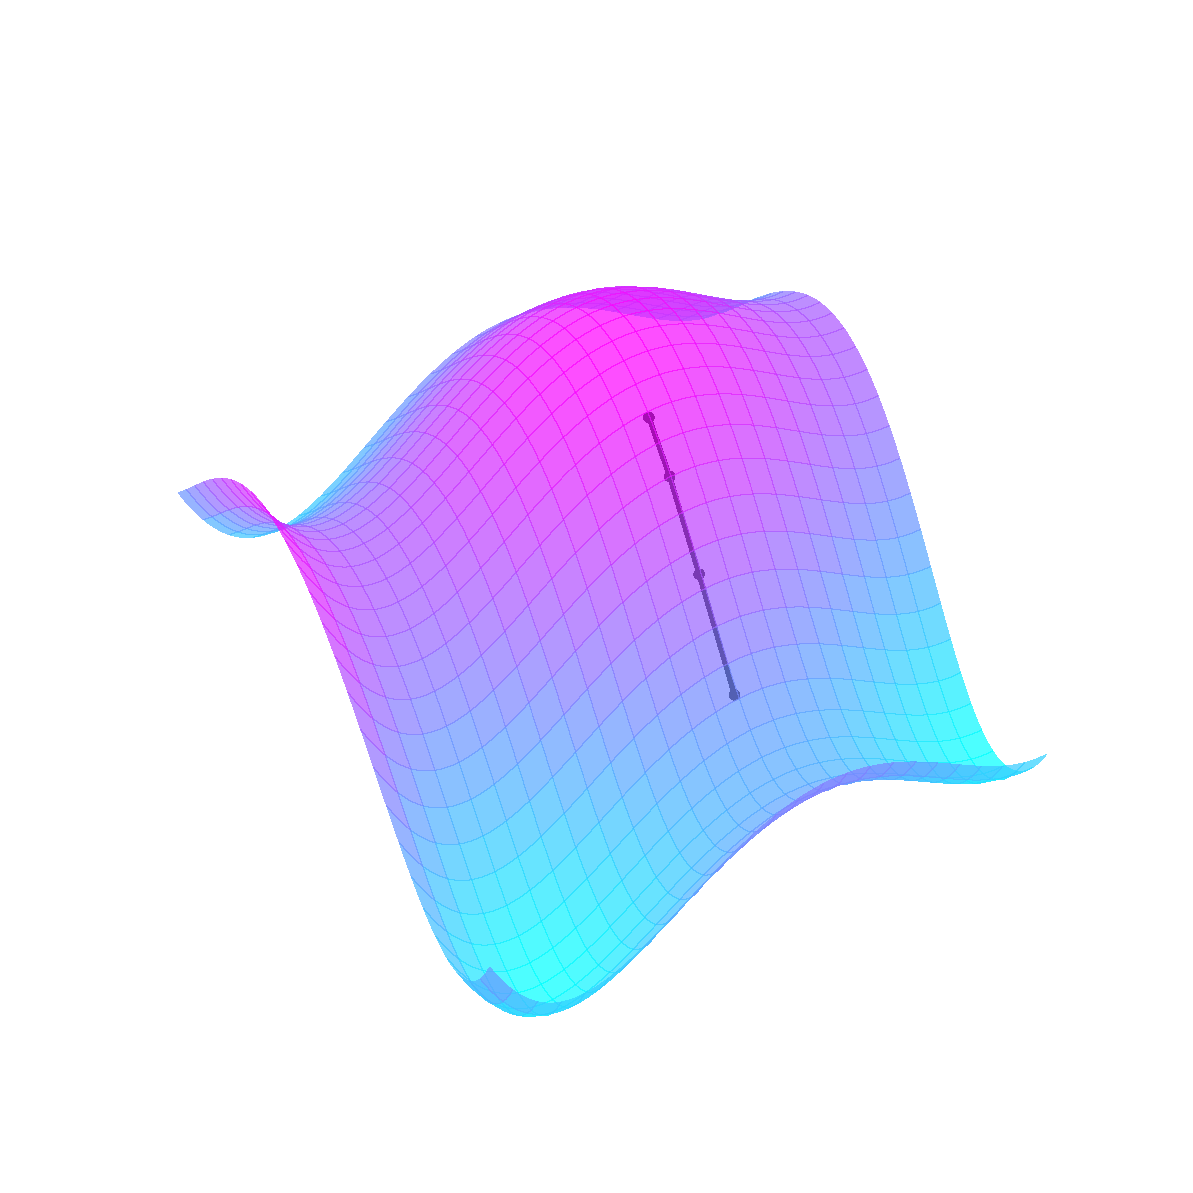
\includegraphics[width=0.8\linewidth]{images/gd_4.pdf}
\end{frame}
\addtocounter{framenumber}{-1}
\begin{frame}
  \centering
  \vspace{1.7em}
  Jusqu'à convergence !

  \vspace{-3.37em}

  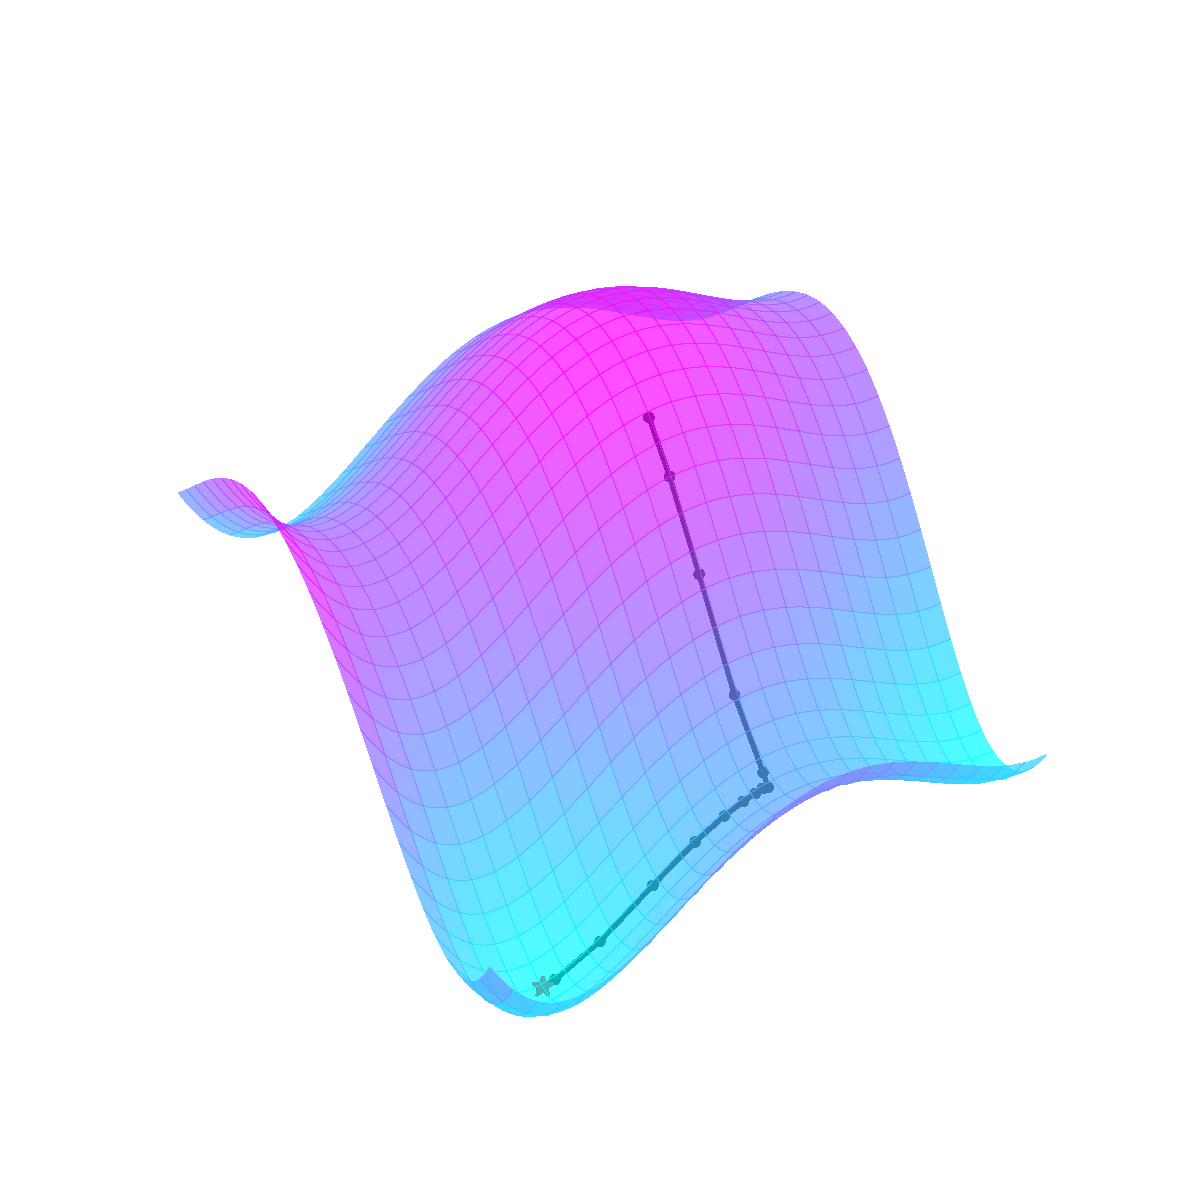
\includegraphics[width=0.8\linewidth]{images/gd_all.pdf}
\end{frame}
\addtocounter{framenumber}{-1}


\subsection{Centralisation des données}
\begin{frame}
  \begin{figure}
    \begin{tikzpicture}
      \node (label) at (0,0){
        \includegraphics[width=0.7\linewidth]{images/gathering_databases.pdf}
      };
      \node (B) at (5.2,-0.1) {modèle appris};
    \end{tikzpicture}
  \end{figure}
\end{frame}

\subsection{Apprentissage}
\begin{frame}
  \begin{figure}
    \begin{tikzpicture}
      \node (label) at (0,0){
        \includegraphics[width=0.7\linewidth]{images/database_learning.pdf}
      };
      \node[text width=4cm] (A) at (0.3,0.5) {algorithmes itératifs (gradient descent etc.)};
      \node (B) at (5.2,-0.1) {modèle appris};
    \end{tikzpicture}
  \end{figure}
\end{frame}

\section{Machine Learning Décentralisé}
\subsection{Principe}
\begin{frame}
  Chacun garde ses données.
  \vspace{1em}
  \begin{figure}
    \includegraphics[width=1\linewidth]{images/mixed_db.pdf}
  \end{figure}
\end{frame}

\begin{frame}
  Graphe de communication fixé.
  \vspace{1em}
  \begin{figure}
    \includegraphics[width=1\linewidth]{images/graph_learn.pdf}
  \end{figure}
\end{frame}


\subsection{Algorithmes}
\begin{frame}
  Itérer jusqu'à convergence :\footcite{lian2017decentralized}
  \begin{itemize}
  \item choisir au hasard un agent $i$ (dont le dataset est $\mathcal D_i$) ;
  \item mise à jour locale :
    \begin{align}
      w_{t}^{(i)} = w_{t}^{(i)} - \gamma \nabla \mathcal L(w_{t}^{(i)}, \mathcal{D}_i)\text{ ;}
    \end{align}
  \item agrégation avec les modèles voisins :
    \begin{align}
      w_{t+1}^{(i)} = \frac{1}{|\mathcal N_i|} \sum_{j\in\mathcal N_i} w_t^{(j)}.
    \end{align}
  \end{itemize}
\end{frame}


\begin{frame}
  Mise à jour locale pour un agent :
  \vspace{1em}
  \begin{figure}
    \begin{tikzpicture}
      \node (label) at (0,0){
        \includegraphics[width=1\linewidth]{images/collaborative_learn_local.pdf}
      };
      \node (A) at (-1.7,-1) {\small $w_{t}^{(i)} = w_{t}^{(i)} - \gamma \nabla \mathcal L(w_{t}^{(i)}, \mathcal{D}_i)$};
    \end{tikzpicture}
  \end{figure}
\end{frame}


\begin{frame}
  Réception des valeurs voisines :
  \vspace{1em}
  \begin{figure}
    \begin{tikzpicture}
      \node (label) at (0,0){
        \includegraphics[width=1\linewidth]{images/collaborative_learn_step1.pdf}
      };
      \node[text width=4cm] (A) at (-1,-1) {$w_{t}^{(2)}$};
      \node[text width=4cm] (A) at (1,1) {$w_{t}^{(4)}$};
      \node[text width=4cm] (A) at (-1,1) {$w_{t}^{(1)}$};
    \end{tikzpicture}
  \end{figure}
\end{frame}

\begin{frame}
  Agrégation des valeurs reçues :
  \vspace{1em}
  \begin{figure}
    \begin{tikzpicture}
      \node (label) at (0,0){
        \includegraphics[width=1\linewidth]{images/collaborative_learn_local.pdf}
      };
      \node[text width=4cm] (A) at (-1.2,-1.2) {\small $\displaystyle w_{t+1}^{(3)} =  \frac{1}{|\mathcal N_3|} \sum_{j\in\mathcal N_i} w_t^{(j)} $};
    \end{tikzpicture}
  \end{figure}
\end{frame}

\section{Confidentialité des Données}
\subsection{Question}
\begin{frame}
  \centering
  La décentralisation suffit-elle a protéger les données locales ?
\end{frame}

\begin{frame}
  \centering
  La décentralisation suffit-elle a protéger les données locales ? \textcolor{CaDarker}{NON.} \footcite{geiping2020inverting}
  \begin{figure}
    \begin{minipage}{.3\textwidth}
      \centering
      \subfloat[Image réelle du dataset.]{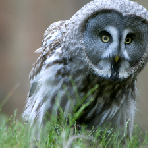
\includegraphics[width=1\linewidth]{images/chouette_reel.png}}%
    \end{minipage}\quad%
    \begin{minipage}{.3\textwidth}
      \centering
      \subfloat[Image reconstruite avant entraînement.]{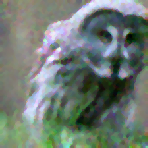
\includegraphics[width=1\linewidth]{images/chouette_untrained.png}}%
    \end{minipage}\quad%
    \begin{minipage}{.3\textwidth}
      \centering
      \subfloat[Image reconstruite après entraînement.]{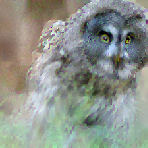
\includegraphics[width=1\linewidth]{images/chouette_trained.png}}%
    \end{minipage}%
    \caption{Reconstruction d'une image $x$ à partir du gradient $\nabla_w \mathcal L_w(x, y)$ d'un réseau de neurones.}
  \end{figure}
\end{frame}

\subsection{Garantir la confidentialité des données}
\begin{frame}
  Differential Privacy \footcite{privacybook} donne une définition de confidentialité.

  \vspace{1em}

  \begin{adjustwidth}{1em}{}
    $\longrightarrow$ Idée : bruiter les informations partagées pour empêcher la reconstruction d'éléments du dataset local.
  \end{adjustwidth}

  \vspace{1em}

  Dans notre algorithme :
  \begin{align}
    w_{t}^{(i)} = w_{t}^{(i)} - \gamma \left(  \nabla \mathcal L(w_{t}^{(i)}, \mathcal{D}_i) + \textcolor{CaDarker}{\eta_t^{(i)}} \right).
  \end{align}

\end{frame}

\subsection{Garantir la confidentialité des données}
\begin{frame}
  Problème : les résultats obtenus ont-ils toujours un sens ?
  \begin{adjustwidth}{1em}{}
    $\longrightarrow$ on peut contrôler le bruit (en proba) ; voir par exemple \footcite{bellet}.
  \end{adjustwidth}

  \begin{theorem}
    Avec $\mathcal J(w) = \mathcal L(w; \mathcal D_1) + \cdots + \mathcal L(w; \mathcal D_n)$ et $w_t = (w_t^1, \dots, w_t^n)$ les itérés générés par notre algorithme. Pour $F$ $\sigma$-fortement convexe, $L$-smooth, avec $\rho = \frac{\sigma}{pL}$ :
    \begin{align}\nonumber
      \mathbb E(\mathcal J(w^T) - \mathcal J^*) \le
      \underbrace{\vphantom{\sum_{t=0}^{T-1}}(1 - \rho)^T \mathbb E(\mathcal J(w^0) - \mathcal J^*)}_{\textcolor{CaDarker}{\text{erreur d'optimisation}}} +
      \underbrace{\sum_{t=0}^{T-1} (1 - \rho)^t \mathbb E(\eta_t^i)^2}_{\textcolor{CaDarker}{\text{bruit additif}}}.
    \end{align}
  \end{theorem}
\end{frame}

\section{Application}
\subsection{Recherche médicale}
\begin{frame}
  Dans le milieu médical, on utilise du ML pour, par exemple :
  \begin{itemize}
  \item études statistiques ;
  \item classification de voix, images...
  \end{itemize}

  \vspace{1em}

  Mais un hôpital n'a pas nécessairement assez de données.
\end{frame}

\begin{frame}
  Partager les données est difficile, car :
  \begin{itemize}
  \item sensibles ;
  \item trop volumineuses ;
  \item leur fuite peut révéler les pratiques d'un service à l'extérieur.
  \end{itemize}

  \vspace{1em}

  $\longrightarrow$ On essaye de proposer une solution avec ML décentralisé privé.
\end{frame}

\section{Conclusion}
\begin{frame}
  Posez toutes vos questions !

  \vspace{1em}

  N'hésitez pas à me contacter :

  \quad \url{paul.mangold@inria.fr}

  \vspace{1em}

  Pour en savoir plus sur Magnet :

  \quad \url{https://team.inria.fr/magnet/}

  \vspace{1em}

  Vous pouvez retrouver ces slides sur

  \quad \url{http://pmangold.fr/presentation/RIC}
\end{frame}



\end{document}